\documentclass[11pt,a4paper]{article}
\synctex=1
\usepackage[utf8]{inputenc}
\usepackage[margin=1cm, bottom=2cm]{geometry}
\usepackage{graphicx}
\usepackage{libertine}
\usepackage{amsmath}
\usepackage{amssymb}
\usepackage{listings}
\usepackage{pgfornament}
\usepackage{eso-pic}
\usepackage{textcomp}
\usepackage{courier}
\usepackage[hangul]{kotex}

\title{
	\centering
	\pgfornament[width=12cm,color=teal]{84}\\
	\vspace{1cm}
	\fontsize{50}{50} \selectfont {자료구조와 실습\\4장 리스트 연습문제}\\
		\pgfornament[width=12cm,color=teal]{88}\\
	\vfill}
\author{
	\LARGE
	\begin{tabular}{rl}
		\hline
		학번 : & 2016110056\\ 
		학과 : & 불교학부 \\
		이름 : & 박승원\\
		날짜 : & \today\\
		\hline
	\end{tabular}\vspace{2cm}
	\\

\includegraphics[width=0.5\textwidth]{logo.jpg}
	}
\date{}


\linespread{1.3}

\begin{document}

\maketitle

%\includegrap

\newpage


\noindent
\begin{enumerate}
	

\item 리스트에 대한 설명 중 틀린 것은?
\begin{enumerate}

	\item 구조체도 리스트의 요소가 될 수 있다.
	\item 리스트의 요소간에는 순서가 있다.
	\item 리스트는 여러 가지 방법으로 구현될 수 있다.
	\item \fbox{리스트는 집합과 동일하다.}
\end{enumerate}

\item 다음은 순차적 표현과 연결된 표현을 비교한 것이다. 설명이 틀린 것을 모두 표시하시오.
	\begin{enumerate}
	\item \fbox{연결된 표현은 포인터를 가지고 있어 상대적으로 크기가 작아진다.}
	\item 연결된 표현은 삽입이 용이하다.
	\item \fbox{순차적 표현은 연결된 표현보다 접근 시간이 많이 걸린다.}
	\item 연결된 표현으로 작성된 리스트를 2개로 분리하기가 쉽다.
	\end{enumerate}
	
\item 다은은 연결 리스트에서 있을 수 있는 여러 가지 경우를 설명한다. 잘못된 항목은?
	\begin{enumerate}
		\item 정적인 데이터보다는 변화가 심한 데이터에서 효과적인 방법이다.
		\item 모든 노드는 데이터와 링크(포인터)를 가지고 있어야 한다.
		\item \fbox{연결 리스트에서 사용한 기억 장소는 다시 사용할 수 있다.}
		\item 데이터들이 메모리상에 흩어져서 존재할 수 있다.
	\end{enumerate}

\item 삽입과 삭제 작업이 자주 발생할 때 실행 시간이 가장 많이 소요되는 자료구조는?
	\begin{enumerate}
		\item \fbox{배열로 구현된 리스트}
		\item 단순 연결 리스트
		\item 원형 연결 리스트
		\item 이중 연결 리스트
	\end{enumerate}

\item 다음 중 NULL 포인터(Null pointer)가 존재하지 않는 구조는 어느 것인가?
	\begin{enumerate}
		\item 단순 연결 리스트
		\item 원형 연결 리스트
		\item \fbox{이중 연결 리스트}
		\item 헤더 노드를 가지는 단순 연결 리스트
	\end{enumerate}

\item 원형 연결 리스트에 대한 설명 중 틀린 것은?
	\begin{enumerate}
		\item 모든 노드들이 연결되어 있다.
		\item 마지막에 삽입하기가 간단하다.
		\item 헤더 노드를 가질 수 있다.
		\item \fbox{최종 노드 포인터가 NULL이다.}
	\end{enumerate}

\item 리스트의 n번째 요소를 가장 빠르게 찾을 수 있는 구현 방법은 무엇인가?
	\begin{enumerate}
		\item \fbox{배열}
		\item 단순 연결 리스트
		\item 원형 연결 리스트
		\item 이중 연결 리스트
	\end{enumerate}
	
\item 단순 연결 리스트의 노드 포인터 p가 마지막 노드를 가리킨다고 할 때, 다음 수식 중 참인 것은?
	\begin{enumerate}
		\item last == NULL
		\item $last\rightarrow data == NULL$
		\item \fbox{$last\rightarrow link == NULL$}
		\item $last\rightarrow link\rightarrow link == NULL$
	\end{enumerate}

\item 단순 연결 리스트의 노드들을 노드 포인터 p로 탐색하고자 한다. p가 현재 가리키는 노드에서 다음 노드로 가려면 어떻게 하여야 하는가?
	\begin{enumerate}
		\item p++;
		\item p$--$;
		\item \fbox{p=p$\rightarrow$ link;}
		\item p=p$\rightarrow $data;
	\end{enumerate}
	
\item 단순 연결 리스트의 관련 함수 f가 헤드 포인터 head를 변경시켜야 한다면 함수 매개 변수로 무엇을 받아야 하는가?
	\begin{enumerate}
		\item head
		\item \fbox{\&head}
		\item *head
		\item head$\rightarrow$link;
	\end{enumerate}
\lstset{language=C, tabsize=4, frame=single, showstringspaces=false, breaklines=true, columns=flexible, basicstyle=\ttfamily\small}


\item A라는 공백 상태의 리스트가 있다고 가정하자. 이 리스트에 대하여 다음과 같은 연산들이 적용된 후의 리스트의 내용을 그려라.
\begin{lstlisting}[frame=none]
add_first(A, "first");
add(A, 1, "second");
add_last(A,"third");
add(A,2,"fourth");
add(A,4,"fifth");
delete(A,2);
delete(A,2);
replace(A, 1, "sixth");
\end{lstlisting}
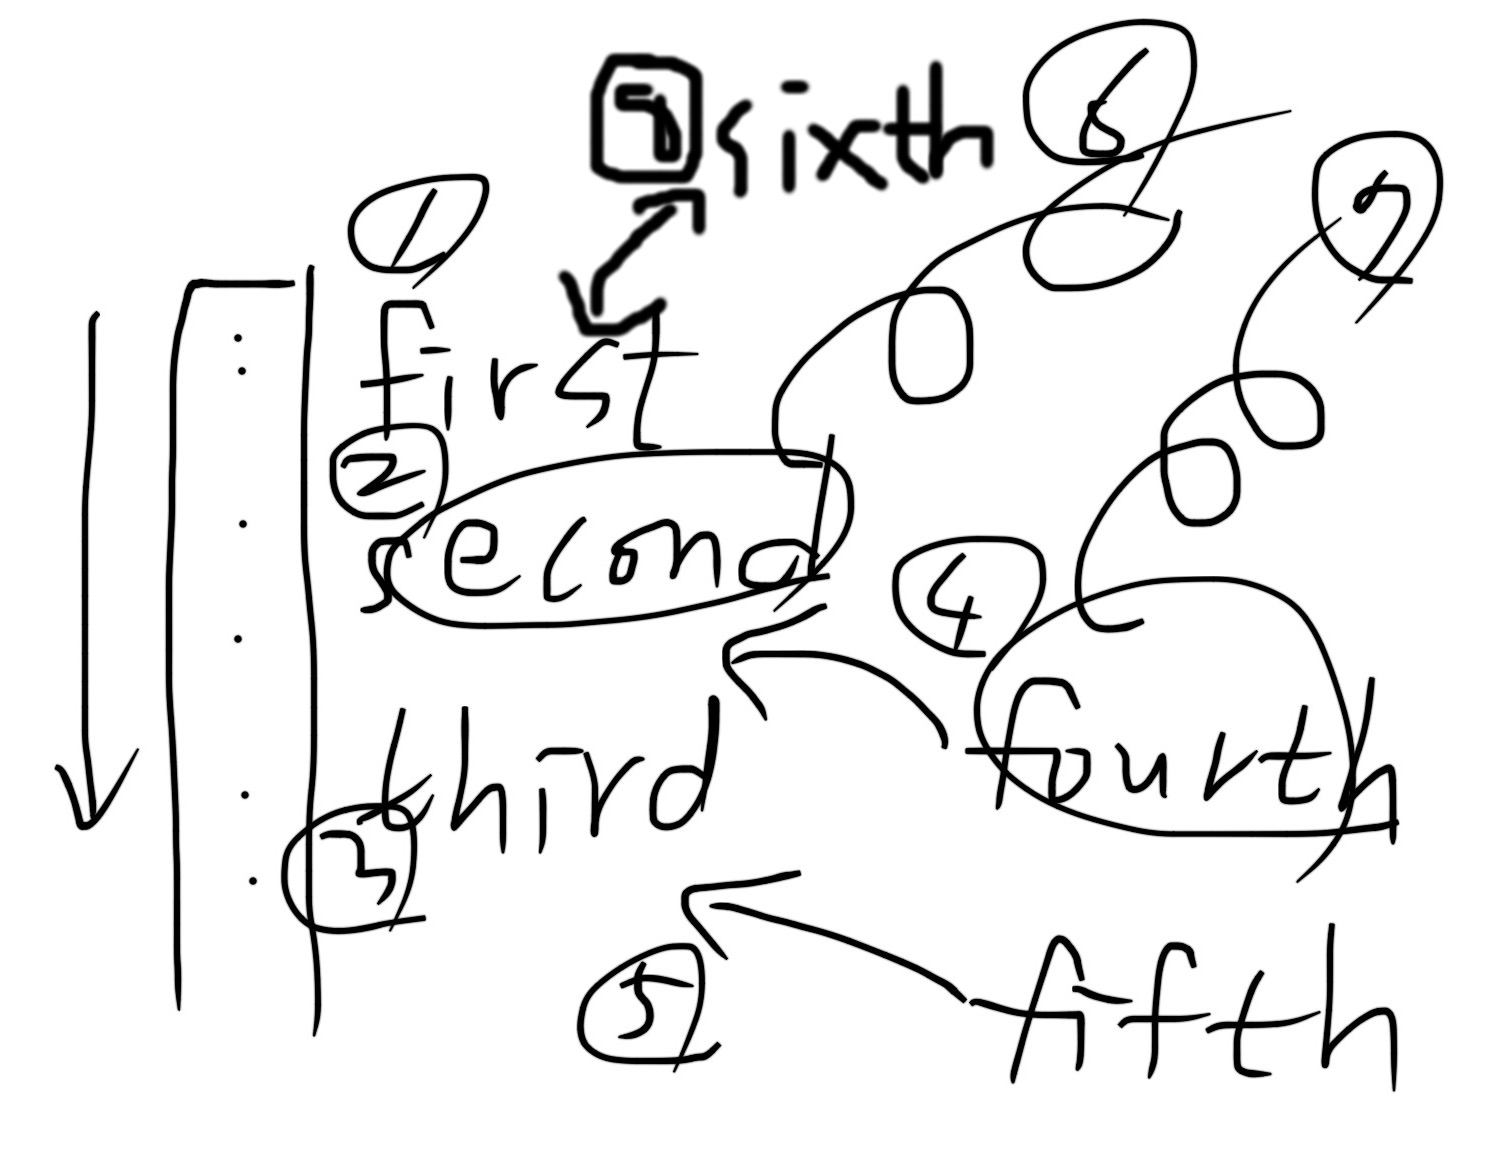
\includegraphics[width=\textwidth]{11.jpg}


\item 배열을 이용하여 구현한 리스트의 경우, 리스트의 연산 중 일부 연산만 구현되어 있다. 본문의 코드를 참조하여 리스트 ADT의 나머지 연산들도 구현하여 보라.
\lstinputlisting{12.c}

\item 단순 연결 리스트에서 삭제 함수 delete 함수는 실제로는 헤드 포인터와 선행 노드 포인터의 2개의 매개변수만 있으면 작성이 가능하다. 이들 두 매개 변수만을 사용하여 다시 작성하라.
\lstinputlisting[language=C, frame=single, title=앞으로 계속 사용하게 될 헤더화일 list.h]{list.h}

\item 단순연결 리스트에 정수가 저장되어 있다. 단순 연결 리스트의 모든 데이터 값을 더한 합을 출력하는 프로그램을 작성하시오.

\item 단순 연결 리스트에서 특정한 데이터 값을 갖는 노드의 개수를 계산하는 함수를 작성하여라.

\item 단순 연결 리스트에서 탐색 함수를 참고하여 특정한 데이터값을 갖는 노드를 삭제하는 함수를 작성하라.

\item 단순 연결 리스트의 헤드 포인터가 주어져 있을 때, 첫 번째 노드에서부터 하나씩 건너서 있는 노드를 삭제하는 함수를 작성하라. 즉, 홀수번째 있는 노드들이 전부 삭제된다.
\lstinputlisting[language=C,frame=single,title=문제 $13\sim17$]{list.c}
\includegraphics[width=0.8\textwidth]{list.png}

\item 두개의 단순 연결 리스트 A,B가 주어져 있을 경우, alternate 함수를 작성하라. alternate 함수는 A와 B로부터 노드를 번갈아 가져와서 새로운 리스트 C를 만드는 연산이다. 만약 입력 리스트 중에서 하나가 끝나게 되면 나머지 노드들을 전부 C로 옮긴다. 함수를 구현하여 올바르게 동작하는지 테스트하라. 작성된 함수의 시간 복잡도를 구하라.
\lstinputlisting[language=C, frame=single]{18.c}

8n+3

\includegraphics[width=0.9\textwidth]{18.png}

\item 원형 연결 리스트에서 헤드 노드를 사용하면 탐색 연산을 조금 빠르게 할수 있다.
즉 원형 연결 리스트에 아무런 역할도 하지 않는 헤드 노드를 하나 추가한다.
탐색 연산을 할 때 찾고자 하는 데이터를 헤드 노드에 미리 저장한다.
헤드 노드 다음 노드부터 탐색을 시작하여 만약 탐색이 헤드 노드에서 끝나게 되면 탐색은 실패한 것이다.
\begin{enumerate}
	\item 다음과 같은 탐색연산을 원형 연결 리스트에 대하여 구현하고 테스트하라.
	\begin{lstlisting}[frame=none]
	ListNode* search(ListNode *head, int data)
	{
		ListNode *current = head->link;
		head->data = data;
		while(current->data != x) {
			current = current->link;
		}
		return ((current == head) ? NULL : current);
	}
	\end{lstlisting}

	\item 이 원형 연결 리스트에서의 탐색 연산 search와 단순 연결 리스트에서의 탐색 연산인 search의 실행 성능을 다음과 같이 비교하라. 
	단순 연결 리스트와 원형 연결 리스트의 크기가 각각 100,1000,10000,100000인 경우의 최악과 평균 실행 시간을 구하여 비교하라. 
	실행 시간이 차이가 나는 이유를 설명하시오.

\end{enumerate}
\lstinputlisting{19.c}
\includegraphics[width=0.9\textwidth]{19.png}

그다지 실행시간에 차이는 없었으나, 헤드를 이용한 탐색의 경우, 시간복잡도가 n이 더 적다. 
즉 헤드가 없을 경우에는 항상 NULL인지 아닌지를 검사하는 과정이 한번 더 소요된다.
\item 두 개의 단순 연결 리스트를 병합하는 함수를 조금 변경하여 보자. 
두개의 연결 리스트 $a=(a_1, a_2,\dots a_n), b=(b_1, b_2, \dots, b_n)$가 데이터 값의 오름차순으로 노드들이 정렬되어 있는 경우, 이러한 정렬 상태를 유지하면서 합병을 하여 새로운 연결 리스트를 만드는 알고리즘 merge를 작성하라. 
a와 b에 있는 노드들은 전부 새로운 연결 리스트로 옮겨진다. 작성된 알고리즘의 시간복잡도도 구하라.
\lstinputlisting{20.c}
\includegraphics[width=0.9\textwidth]{20.png}

7n+3

\item 보통 연결 리스트에서는 선행 노드를 알아야만이 노드를 삭제할 수 있다.
	그러나, 다음과 같이 하면 선행 노드를 모르고도 노드를 삭제할 수 있다. 
	먼저 원형 연결 리스트라고 가정하자. 
	어떤 노드를 가리키는 포인터 x가 주어진 경우, 그 노드의 후속 노드를 쉽게 찾을 수 있다.
	후속 노드를 y라고 한다면 x에 y의 데이터 필드값을 복사한다. 
	그리고 y를 삭제한다. 
	그러면 실질적으로는 x가 삭제된 것처럼 된다. 
	이런 식으로 노드를 삭제하는 함수 remove\_node2를 작성하고 구현하여 테스트하라.
\lstinputlisting[language=C,frame=single]{21.c}
\includegraphics[width=0.9\textwidth]{21.png}

\item 단순 연결 리스트 C를 두개의 단순 연결 리스트 A와 B로 분리하는 함수 split를 작성하여 보자. C의 홀수번째 노드들은 모두 A로 이동되고 C의 짝수번째 노드들은 모두 B로 이동된다. 이 함수가 C를 변경하여서는 안된다. 작성된 알고리즘의 시간 복잡도를 구하고 구현하여 수행하여 보자.
\lstinputlisting[language=C, frame=single]{22.c}
\includegraphics[width=0.9\textwidth]{22.png}

\item 두 개의 다항식이 다음과 같이 주어졌다. 이들을 연결 리스트를 이용하여 나타내고 본문의 프로그램을 이용하여 두 다항식의 합을 구해보시오.

$A(x)=2x^6+7x^3-2x^2-9, B(x)=-2x^6-4x^4+6x^2+6x+1$

\item 다항식을 연결 리스트로 표현할 수 있음을 보였다.
다항식이 연결 리스트로 표현되어 있고, p를 다항식을 가리키는 포인터라고 할 때, 어떤 실수 x에 대하여 이 다항식의 값을 계산하는 함수 poly\_eval을 작성하라.
즉, 다항식이 $x^3+2x+6$이고, x=2이면 $2^3+2*2+6$를 계산하는 함수를 작성하여보라.

\item 다항식이 연결 리스트로 표현되어 있는 경우, 두 개의 다항식을 받아서 다항식의 뺄셈을 수행하는 함수 poly\_sub를 작성하라.
\lstinputlisting[title=문제 $23\sim25$]{23.c}
\includegraphics[width=0.9\textwidth]{23.png}

\item 다음의 연산에 대해 이중 연결 리스트가 단일 연결 리스트보다 좋은 점이 있는가를 설명하라.
\begin{enumerate}
	\item 각 노드를 처리하기 위해 리스트를 순회한다.
	\item loc 위치에 있는 노드를 삭제한다.
	\item \fbox{loc의 위치에 있는 노드 바로 앞에 새 노드를 삽입한다.}
	\item loc의 위치에 있는 노드 바로 뒤에 새 노드를 삽입한다.
\end{enumerate}
	
\item 배열을 이용하여 숫자들을 입력 받아 항상 정렬된 상태로 유지하는 리스트 SortedList를 구현하여 보라. 다음의 연산들을 구현하면 된다.

ADT 4.2 SortedList
\begin{itemize}
	\item 객체 : n개의 element형으로 구성된 순서있는 모임.
	\item 연산 :
	
	add(list, item) ::= 정렬된 리스트에 요소를 추가한다.\\
	delete(list, item) ::= 정렬된 리스트에서 item을 제거한다.\\
	clear(list) ::= 리스트의 모든 요소를 제거한다.\\
	is\_in\_list(list, item) ::= item이 리스트 안에 있는지를 검사한다.\\
	get\_length(list) ::= 리스트의 길이를 구한다.\\
	is\_empty(list) ::= 리스트가 비었는지를 검사한다.\\
	is\_full(list) ::= 리스트가 꽉찼는지를 검사한다.\\
	display(list) ::= 리스트의 모든 요쇼를 표시한다.
\end{itemize}

\lstinputlisting{27.c}
\includegraphics[width=0.9\textwidth]{27.png}

\item 단순 연결 리스트를 이용하여 숫자들을 항상 정렬된 상태로 유지하는 리스트 SortedList를 구현하여 보자.
앞의 문제의 연산들을 구현하면 된다.
\lstinputlisting{28.c}
\includegraphics[width=0.9\textwidth]{28.png}

\item 이중 연결 리스트를 이용하여 숫자들을 항상 정렬된 상태로 유지하는 리스트 SortedList를 구현하여 보자.
앞의 문제의 연산들을 구현하면 된다.
\lstinputlisting{29.c}
\includegraphics[width=0.9\textwidth]{29.png}

\item 본문에서 언급한 대로 연결 리스트에서 헤더 노드(header node)의 개념을 사용하는 것은 상당한 장점이 있다. 먼저 어떤 장점이 있는지를 말하고 단순 연결 리스트의 함수들을 다음과 같은 헤더 노드의 포인터를 받아서 연산을 수행하도록 변경하여 보라.
\lstinputlisting{30.c}
단순연결 리스트에서 리턴값을 잘 이용하고, 재귀함수를 잘 활용하면, 매우 간단하고 깔끔하게 리스트를 작성할 수 있다. 헤더노드 없이도 충분히 가능한데, 헤더노드를 사용하면 프로그램이 약간 지저분해 지는 느낌이 들지만, 프로그래밍적 편의성 면과 실행 성능 측면에서는 더 낫다. 단순연결리스트의 장점은 매우 직관적이고 간명한 프로그램을 짤 수 있다는 것이다.
\item 행렬은 숫자나 문자를 정사각형 또는 직사각형으로 배열하여 그 양끝을 괄호로 묶은 것으로 많은 문제를 수학적으로 해결하는 도구이다. 희소 행렬(sparce matrix)은 많은 항들이 0인 행렬이다. 
연결리스트를 이용하여 희소행렬을 표현하는 방법을 생각하여 보고 구현하라.
\begin{lstlisting}
struct SparseMatrix {//첫번째 노드에서는 행렬의 너비 높이 0이 아닌 값의 갯수이고, 
	int x, y, v;//두번째 노드부터는 x,y좌표와 그 값이다.
	struct SparseMatrix* node;
} SparseMatrix;
\end{lstlisting}
\lstinputlisting[title=리스트를 활용한 Line Editor]{lineeditor.c}
\includegraphics[width=0.8\textwidth]{line.png}
\end{enumerate}

\vspace{2cm}
{\Huge 소감}

리턴값을 잘 활용하면 리스트를 깔끔하게 만들 수 있다. 리스트는 재귀함수를 많이 활용할 수 있는 부분이었다. 포인터를 다루는 것은 아직도 많이 실수를 유발한다. 리스트를 좀 더 활용해 보기 위해 라인에디터를 직접 만들어 보았다. 라인을 삽입시에 개행문자가 하나 끼어드는 버그가 있다. 왜 그런지 잘 모르겠다. scanf를 fgets로 바꾸어 보기도 했는데 해결이 안된다.

\end{document}
